%%
%%
%% The first command in your LaTeX source must be the \documentclass
%% command.
%%
%% For submission and review of your manuscript please change the
%% command to \documentclass[manuscript, screen, review]{acmart}.
%%
%% When submitting camera ready or to TAPS, please change the command
%% to \documentclass[sigconf]{acmart} or whichever template is required
%% for your publication.
%%
%%
\documentclass[sigconf,screen,review,anonymous]{acmart}

\usepackage{multirow}
\usepackage{svg}
\usepackage{xcolor}

\newcommand{\todo}[1]{\textcolor{red}{\textbf{[TODO:#1]}}}

%%
%% \BibTeX command to typeset BibTeX logo in the docs
\AtBeginDocument{%
  \providecommand\BibTeX{{%
    Bib\TeX}}}

%% Rights management information.  This information is sent to you
%% when you complete the rights form.  These commands have SAMPLE
%% values in them; it is your responsibility as an author to replace
%% the commands and values with those provided to you when you
%% complete the rights form.
\setcopyright{acmcopyright}
\copyrightyear{2024}
\acmYear{2024}
\acmDOI{XXXXXXX.XXXXXXX}

%% These commands are for a PROCEEDINGS abstract or paper.
\acmConference[FSE '24]{The 32nd ACM Symposium on the Foundations of Software Engineering}{November 15--19, 2024}{Porto de Galinhas, Brazil}
%%
%%  Uncomment \acmBooktitle if the title of the proceedings is different
%%  from ``Proceedings of ...''!
%%
\acmBooktitle{Proceedings of the 32nd ACM Symposium on the Foundations of Software Engineering (FSE '24), November 15--19, 2024, Porto de Galinhas, Brazil}
\acmPrice{15.00}
\acmISBN{978-1-4503-XXXX-X/18/06}


\settopmatter{printacmref=false}
\renewcommand\footnotetextcopyrightpermission[1]{}

%%
%% Submission ID.
%% Use this when submitting an article to a sponsored event. You'll
%% receive a unique submission ID from the organizers
%% of the event, and this ID should be used as the parameter to this command.
%%\acmSubmissionID{123-A56-BU3}

%%
%% For managing citations, it is recommended to use bibliography
%% files in BibTeX format.
%%
%% You can then either use BibTeX with the ACM-Reference-Format style,
%% or BibLaTeX with the acmnumeric or acmauthoryear sytles, that include
%% support for advanced citation of software artefact from the
%% biblatex-software package, also separately available on CTAN.
%%
%% Look at the sample-*-biblatex.tex files for templates showcasing
%% the biblatex styles.
%%

%%
%% The majority of ACM publications use numbered citations and
%% references.  The command \citestyle{authoryear} switches to the
%% "author year" style.
%%
%% If you are preparing content for an event
%% sponsored by ACM SIGGRAPH, you must use the "author year" style of
%% citations and references.
%% Uncommenting
%% the next command will enable that style.
%%\citestyle{acmauthoryear}


%%
%% end of the preamble, start of the body of the document source.
\begin{document}

%%
%% The "title" command has an optional parameter,
%% allowing the author to define a "short title" to be used in page headers.
\title{RAX: A porting complexity evaluation tool for RISC-V}

%%
%% The "author" command and its associated commands are used to define
%% the authors and their affiliations.
%% Of note is the shared affiliation of the first two authors, and the
%% "authornote" and "authornotemark" commands
%% used to denote shared contribution to the research.
\author{Yuxuan Wang}
\email{wangyuxuan22@otcaix.iscas.ac.cn}
\affiliation{%
  \institution{Institute of Software, Chinese Academy of Sciences}
  \city{Haidian}
  \state{Beijing}
  \country{China}
}

%%
%% By default, the full list of authors will be used in the page
%% headers. Often, this list is too long, and will overlap
%% other information printed in the page headers. This command allows
%% the author to define a more concise list
%% of authors' names for this purpose.
\renewcommand{\shortauthors}{Yuxuan et al.}

%%
%% The abstract is a short summary of the work to be presented in the
%% article.
\begin{abstract}
In recent years, RISC-V instruction set architecture(ISA) has attracted the attention of the information technology industry due to its open source, modular design, and simplicity.
However, there is a lack of standardized metrics and methods to measure software architecture portability, which helps to establish a mature software ecosystem in RISC-V.
A theoretical framework is urgently needed as a guide to summarize important porting-related factors and design an automated RISC-V-oriented porting complexity evaluation tool to solve the problem.
We propose RAX, it will help recommend software with varying degrees of porting complexity to development teams.
RAX first retrieves porting modification information of the adapted project according to the Git version control tool, classifies it through manual analysis, and selects the most important porting factors to design the code positioning mode.
Additionally, it incorporates Cyclomatic Complexity, which is from code evaluation domain, to enhance assessment accuracy and measure the overall complexity of the software.
We establish a high-quality data set of software porting complexity, and select random forest machine learning model as the final classifier through multi-model comparison.
\end{abstract}

%%
%% The code below is generated by the tool at http://dl.acm.org/ccs.cfm.
%% Please copy and paste the code instead of the example below.
%%
\begin{CCSXML}
<ccs2012>
    <concept>
        <concept_id>10011007.10011006.10011072</concept_id>
        <concept_desc>Software and its engineering~Software libraries and repositories</concept_desc>
        <concept_significance>500</concept_significance>
        </concept>
    <concept>
        <concept_id>10011007.10011074.10011111</concept_id>
        <concept_desc>Software and its engineering~Software post-development issues</concept_desc>
        <concept_significance>300</concept_significance>
    </concept>
</ccs2012>
\end{CCSXML}
  
\ccsdesc[500]{Software and its engineering~Software libraries and repositories}
\ccsdesc[300]{Software and its engineering~Software post-development issues}


%%
%% Keywords. The author(s) should pick words that accurately describe
%% the work being presented. Separate the keywords with commas.
\keywords{ISA(Instruction set architecture), RISC-V, Porting Complexity Evaluation}

%% A "teaser" image appears between the author and affiliation
%% information and the body of the document, and typically spans the
%% page.
%% \begin{teaserfigure}
%%  \includegraphics[width=\textwidth]{sampleteaser}
%%  \caption{Seattle Mariners at Spring Training, 2010.}
%%  \Description{Enjoying the baseball game from the third-base
%%  seats. Ichiro Suzuki preparing to bat.}
%%  \label{fig:teaser}
%% \end{teaserfigure}

%% \received{20 February 2007}
%% \received[revised]{12 March 2009}
%% \received[accepted]{5 June 2009}

%%
%% This command processes the author and affiliation and title
%% information and builds the first part of the formatted document.
\maketitle

\section{Introduction}
RISC-V is an emerging open-source and reduced ISA which avoids potential risks such as intellectual property issues\cite{2014The}.RISC-V provides an alternative to traditional commercial instruction set architectures. OpenCloudOS Kernel Stream 2207.2 kernel version adds support for the RISC-V 64 architecture\cite{osti_1560133}; openEuler has joined RISC-V International, and RISC-V has officially become openEuler's official support architecture.The RISC-V SIG took the lead in completing the mainline integration of openEuler RISC-V 23.09\cite{osti_1560132}.

Although RISC-V has already made initial progress in having a relatively complete tool chain, it still requires the support of a large number of application software \cite{2019Notary}.
However, establishing a mature software ecosystem still face challenges.
Currently, there is a lack of standardized metrics to measure software architecture portability,and porting planning relies on domain expertise.The difficulty in estimating porting work leads to challenges in accurately allocating resources;In the context of varying levels of developers' skills in porting, there is an even greater need to efficiently assess the difficulty of software package porting and provide guidance to developers of all kinds.In order to solve these problems,one of the methods is to make analogies with adapted projects to gain porting experience,but it is difficult to extract factors by manual sorting;Even if developers have sensitivity to architecture-related modules, it is still challenging to accurately obtain the workload. 
Du Jiman et al. have developed a basic statistical evaluation plan for CPU architecture code in project \cite{2023du}, however, their work lacks a thorough validity analysis and comparison of factors,and fails to consider the complexity associated with the software operation and maintenance process.

RAX can provide developers with accurate evaluation, recommend software with different levels of porting difficulty based on their skill levels.
The contributions of this paper are as follows:
\begin{enumerate}
  \item Firstly, we conducted analysis on selection of factors related the porting evaluation,investigated the significance of code complexity metrics in the context of porting work and incorporated Cyclomatic Complexity as a factor to assess the overall complexity of  the project.
  \item Based on porting-related factors, we designed a scanning tool to collect porting complexity vectors and ultimately selected random forest machine learning model as the classifier for RAX.
  \item Evaluate the effectiveness of RAX.
  We nearly doubled the dataset compared to Du Jiman's tool,and verified the effectiveness of the evaluation of 100 extension projects in real porting scenarios through their respective communities or forums. We received 50 valid responses.Our findings indicate that RAX outperforms the Du Jiman's tool, delivering substantial improvements in terms of performance and accuracy..
\end{enumerate}


\section{RAX}
The following is an introduction to the process of RAX construction, as shown in Figure \ref{fig:flow-chart}.
During the analysis phase,architecture-related factors are obtained through the Commit tool for selection.
A scanning tool is built to get potential modification workload.
Finally,an appropriate machine learning model is selected as a classification.

\begin{figure}
  \centering
  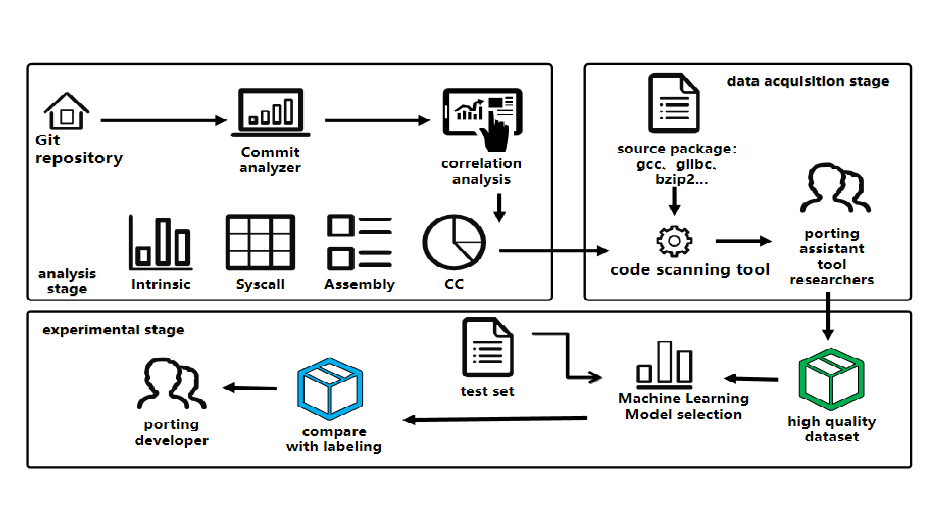
\includegraphics[width=\linewidth]{flow-chart.pdf}
  \caption{Flow chart for method to build RAX}
  \label{fig:flow-chart}
  \Description{Flow chart for method to build RAX}
\end{figure}

\subsection{Motivation}
The section provides a validity analysis of porting-related factors on RAX.
First,we use code complexity metrics to evaluate porting work.
The software metrics of code Cyclomatic Complexity(CC) can help developers make macro judgments on software complexity and maintenance difficulty, evaluate potential and hidden porting difficulties, and help the tool improve accuracy \cite{2005Exploring}.
At present, CC indicators are mostly used in project code quality assessment, defect inspection, code reconstruction, etc \cite{1991Cyclomatic}.
During the porting process, developers will target a large number of project source codes, scripts, assembly codes,and a macro understanding of the project is required in the early stage of porting.
This part of the work has a lot of overlap with the scope of code complexity.

\subsubsection{Factor 1: Cyclomatic Complex(CC)}
\label{sec:factor-1}
RAX tool uses the lizard CC detection tool and optimize its functions,we will introduce it in Section \ref{sec:method}.
This study analyzes the relationship between CC and software porting complexity using the Spearman Rank correlation coefficient analysis method.
We invited five Master's students who are engaged in research on porting auxiliary tools to score the porting complexity(score) of 131 software adapted for RISC-V,collected from the OpenEule list and GitHub.
According to the collection of Internet events, log analysis, source code dismantling, and similar project analogy \cite{liangguanyu2020}, we form a scoring interval in the range of $[0~5]$.
We then calculated the Spearman correlation coefficient and conducted significance analysis between score and the CC factors.
The Spearman coefficient is 0.608, with a P-value of 1.39e-14, which is less than 0.01.
This indicates a significant correlation between the two variables.
The results suggest that CC has a moderate positive correlation with porting difficulty.
This is because developers need a holistic understanding of the project during the porting process, and CC can represent the overall complexity of the project, potentially reflecting porting barriers, as shown in Figure \ref{fig:relationship}.
Secondly,we focus on the code associated with architecture in the project,with the goal of predicting porting workload through these code.

\begin{figure}
  \centering
  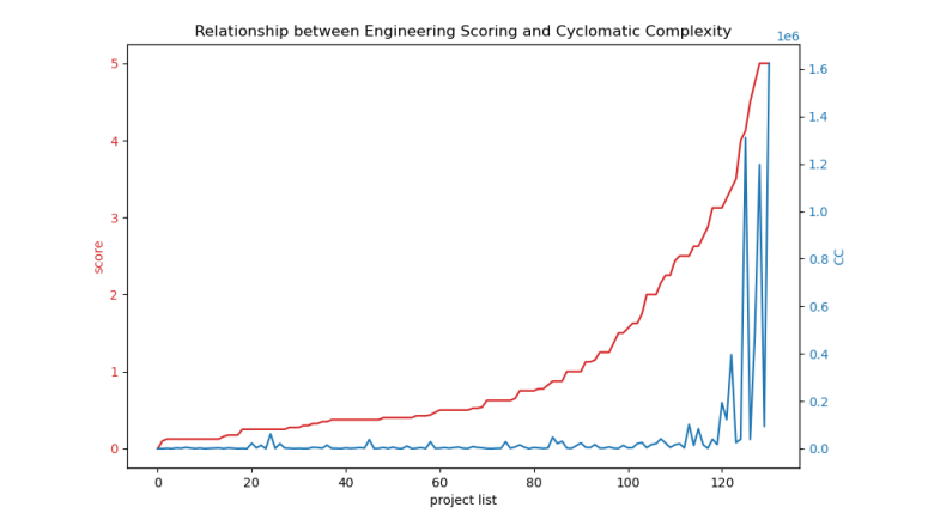
\includegraphics[width=\linewidth]{relationship.pdf}
  \caption{The relationship between score and CC}
  \label{fig:relationship}
  \Description{The relationship between score and CC}
\end{figure}

\subsubsection{Factor2:Arch\_code}

First, extract all possible architecture-related factors.
Use the Git tool to split Commit into different files using git-diff and filter out the surrounding 20 lines of content containing architecture keywords for detailed analysis of the modifications.
The manually analyzed Commit generally includes the following parts: first, functional supplements, including lack of dependent package calls, performance optimization and test cases for architecture porting;second, detail adjustments for data type and Build script;finally, key function implementation, assembly code, built-in function, system call, etc.
Among these factors, we select more objective ones that can be automatically located through regular expression matching.

Arch\_code defines assembly code, conditional compilation and macro structure, Intrinsic functions, Builtin functions, architecture-related build scripts, and system calls.
We use an automated architecture binding code scanning module to obtain statistics on the number of lines and frequencies of Arch\_code.

Continue to collect other factors that may affect the evaluation of porting complexity,and select the following parameters through the Commit analyzer:architecture-related code lines, architecture-related files, and architecture keywords.
The number of architecture-related code lines and files is located using the keywords of X86, ARM, MIPS, RISCV, SPARC and other architectures.
%Correlation comparison between Arch\_code and other factors acquired by Commit analyzer,as shown in Table \ref{tab:score}:

%\begin{table}
 % \caption{The Spearman correlation coefficient of score and architecture-related factors}
  %\label{tab:score}
  %\begin{tabular}{cc}
   % \toprule
    %Type & Score \\
    %\midrule
    %conditional compilation & 0.73 \\
    %Builtin & 0.61 \\
    %Intrinstic & 0.74 \\
    %syscall & 0.69 \\
    %asm & 0.66 \\
    %build\_scripts & 0.43 \\
    %time & -0.16 \\
    %authors & 0.43 \\
    %lines of arch & 0.16-0.40 \\
    %files of arch & 0.34-0.41 \\
    %keyword count & 0.17-0.43 \\
   % \bottomrule
  %\end{tabular}
%\end{table}
Correlation comparison between Arch\_code and other factors acquired by Commit analyzer,as shown in Figure \ref{fig:correlation}:
\begin{figure}
  \centering
  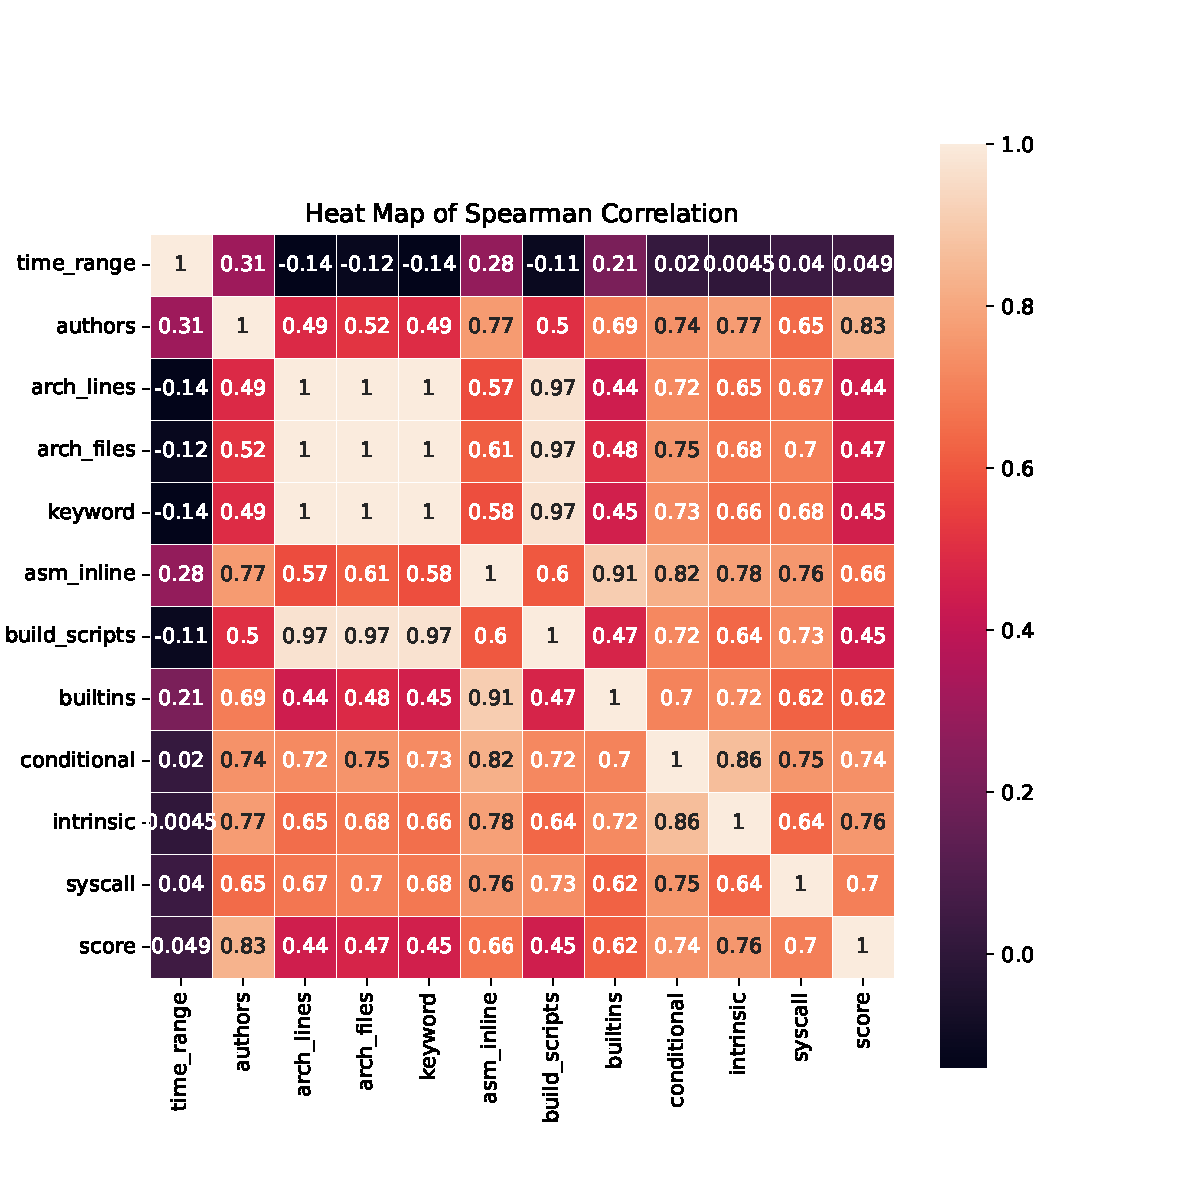
\includegraphics[width=\linewidth]{correlation.pdf}
  \caption{The Correlation}
  \label{fig:correlation}
  \Description{The Correlation}
\end{figure}


The results indicate that Arch\_code has a higher correlation with score compared to other factors, and it also aligns with the significant results of the Spearman correlation test.
The use of only architecture keywords for statistics yields moderate effectiveness in evaluating tool because keywords can only be detected from comments and macro sections of Commit, while critical porting code may lack these keywords,but the keyword count can reflect the amount of porting modification from the side.
As shown in the figure 2, there may be great ambiguity in keyword positioning using different architectures.
So we only selected x86 for positioning, which represents the most fair workload.
In the end, the parameters of Arch\_code show a correlation of 0.43 to 0.75 with score, indicating a strong relationship.
However, using a single factor alone does not result in a significantly strong correlation, as the combined modifications of these factors make up the porting workload.

To design RAX that assists developers with porting work,the following research questions are proposed:

\textbf{Research Question 1:} Developers often struggle to make fine-grained differentiations in the complexity of porting projects.
How can we select architecture-relevant factors to design an automated tool that assesses the porting difficulty?
We analyzes the porting modifications obtained from developer Commit in the Git tool.
We conducts an effectiveness analysis of the selected factors and filters out strongly correlated ones that can be automatically identified using the Lines of Code (LOC) approach.
Additionally, we propose a CC assessment method to jointly establish a data set for porting complexity.

\textbf{Research question 2:} How to select a classifier to obtain effective classification results for the tool?
Using the processing method of unbalanced datasets, multiple machine learning models are compared to select the final classifier.

\subsection{Dataset}
We used the project upstream warehouse to build the data set,that projects mainly targeting C and C++ are from the OpenEuler\citep{stage2023} list and GitHub,and invited 5 postgraduate students who are engaged in the research of RISC-V porting auxiliary tools to participate in the experimental evaluation.Specific evaluation methods can be found in 2.1.1. The evaluation scores are divided into three categories: low, medium, and high\citep{githuburl}.This includes 139 projects as training, testing, and validation datasets, while more than 80 additional projects were used as a tool evaluation dataset. To gather insights from developers, the community, forums, and emails were utilized, resulting in over 50 meaningful feedback responses. In order to address the issue of data imbalance caused by collecting datasets solely from the openEuler mailing list, where more than 80\% of the projects were initially evaluated as having low porting complexity, a greater emphasis was placed on projects that had higher numbers of likes on GitHub and were deemed more important and active. Additionally, efforts were made to collect projects from the bottom such as operating systems, kernel-level projects,mathematical computation libraries,and machine learning libraries.

\subsection{Method}
\label{sec:method}
The RAX combines the CC calculation module and the Arch\_code location module to obtain the porting vector,and the complexity vector and score together form the data set.

\subsubsection{Lizard CC calculation module}
Lizard's default computing method is basically consistent with McCabe's theory \cite{1702388}.
However, Lizard tool only detects defects at the function level and uses the average function CC for file-level statistics, which is not suitable for current porting complexity detection requirements \cite{9402593}.
This paper proposes a new method for evaluating CC specifically for porting assessment work:
\begin{enumerate}
  \item First, calculate the function-level CC for all files in the project using McCabe's method.
  \item Following Liu Huihui's mention of System Cyclomatic Complexity (SCC) in software evolution assessment techniques based on code change detection \cite{liuhuihui00}, we define SCC as the total sum of function-level values in the system.
  The advantage is that it can avoid the use of overly complex methods, which will cause deviations to affect the classification results.
  Additionally, it eliminates the problem of decreased detection performance caused by program transformation into syntax abstract trees and control flow graphs.
\end{enumerate}

\subsubsection{Arch\_code location module}
we form the Arch\_code dictionary:
\begin{enumerate}
  \item Conditional compilation and architecture macros are used as preprocessor macros to enable projects to select execution on different hardware architectures, thus demonstrating the additional workload of architecture porting.
  Use conditional compilation statements, such as ``if defined'', ``ifdef'', in conjunction with all possible architectur macros,``\_\_x86\_64\_\_''.
  We use a similar bracket matching algorithm to cover all the code within macros, avoiding the impact of nested layers.
  Additionally, we only collect the keyword dictionary for x86 architecture.
  This is because different architectures may reflect varying workloads and difficulties, while considering that multiple architectures blurs the classification performance in practical work.
  \item Assembly code Leverages the advantages of architecture-specific instructions to enhance performance.
  Considering that architecture changes inevitably require consideration of the assembly section, we use matching forms such as ``\_\_asm\_\_'' and ``\_\_volatile\_\_''.
  In future work,we will consider striving to achieve the currently unachievable architecture identification function of assembly code and identify assembly code in the form of instructions;In actual work, the assembly code of different architectures may represent different levels of difficulty.
  For example, the assembly code of ARM is relatively simple.
  At the same time,there are also situations where some assembly codes only need to serve a specific architecture and do not need to be fully modified when porting to RISC-V.
  This is why we cannot achieve Fine-grained evaluation,we simply count the number of lines.
  \item Intrinsic functions are interfaces provided by compilers that are closely related to the architecture.
  Calling Intrinsic functions can replace assembly code.
  We compile dictionaries of Intrinsic functions based on official documentation from x86.
  Builtin function also employ a similar approach;In the future,we may assign difficulty weights to them.
  Currently,we only perform frequency statistics on them.
  Additionally,we will continue to supplement the analysis of whether the functions already have corresponding implementation for RISC-V and whether they are truly needed in RISC-V.
  \item System calls are encapsulated by the operating system kernel to provide hardware calling.
  Considering glibc's support for system call encapsulation, reorganize the sys-call dictionary.
  The system calls that do not support RISC-V have been filtered out currently.
  \item In the porting process, adjustment of build scripts is necessary to ensure smooth compilation.
  We locate architecture keywords in the build scripts.
  In the future, architecture-related factors will consider even finer-grained classification.
  For instance,considering the impact of existing porting auxiliary tools, including intrinsic translation tools and assembly translation tools,on porting complexity assessment.
\end{enumerate}

\section{Result and analysis}

To answer research question 2, based on the work of Chen Xiang et al. \cite{5128907}, aiming at the status quo of unbalanced datasets and small sample datasets, we try to use ensemble learning methods \cite{6509481}, SMOTE \cite{4271036}, and random oversampling methods for data preprocessing.
Ultimately, we chose to train four models: Random Forest, Support Vector Machine, Adaboost, and Xgboost.
By comparing multiple indicators, we select the Random Forest machine learning as the classifier.

\begin{table}
  \caption{ Experimental results of models}
  \label{tab:evaluation}
  \begin{tabular}{ccccc}
    \toprule
     & Accuracy & Pmacro & Rmacro & F1macro \\
    \midrule
    Adaboost & 0.786 & 0.594 & 0.775 & 0.650 \\
    Random Forest & 0.857 & 0.817 & 0.873 & 0.836 \\
  \bottomrule
\end{tabular}
\end{table}

We continued to expand 100 projects as a supplementary data set, of which 87 were able to predict correctly.
The prediction results were determined through comments from the community and forums.
Appendix presents a comparative assessment of the porting complexity evaluation tool developed by Du Jiman et al. across various projects.Through real-world evaluations within the developer community, our tool has exhibited a significant improvement in accuracy, surpassing other comparable tools by a margin of 14\%. In the appendix, we provide a comprehensive compilation of the community's valuable feedback comments, accompanied by the relevant web links for further reference and validation.

\begin{table}
  \caption{Effectiveness comparison chart}
  \label{tab:effectiveness}
  \begin{tabular}{ccccc}
    \toprule
    Porting Complexity & \multicolumn{2}{c}{Du's Tool} & \multicolumn{2}{c}{RAX} \\
     & TP & FN & TP & FN \\
    \midrule
    Low &31/36 & 5/36 & 34/36 & 2/36 \\
    Medium & 5/8 & 3/8 & 6/8 & 2/8 \\
    High & 3/6 & 3/6 & 6/6 & 0/6 \\
    \midrule
    Total & \textcolor{red}{39/50} & 11/50& \textcolor{red}{46/50} & 4/50 \\
      \bottomrule
\end{tabular}
\end{table}

After adding the code complexity factor and modifying the original tool design model, RAX's result prediction accuracy is improved.
This is because code complexity can effectively distinguish projects with low porting difficulty from projects with medium and high porting difficulty.
Motivation Chapters present the cause analysis.
Adding factors also makes RAX more robust and more friendly to projects with unbalanced complexity vectors.
For example, kernel-level projects, boot layers, hardware drivers and other projects may involve a large amount of assembly code,corresponding to larger porting complexity,but other factors of the original tool design are at low values,which is not conducive to distinguishing complexity.
Chibios,u-boot are facing such a situation.
Within this assessment, there are instances of inaccurate predictions.


In-depth analysis of these variations reveals that certain projects exhibit inherent complexity, entailing a substantial presence of architecture-specific code defined by Arch\_code.
Nevertheless, the practical porting process benefits from an array of auxiliary tools designed to support developers. In response to valuable suggestions from developers within the OpenEuler community, we conducted an evaluation of the porting difficulty for various versions of the Chromium.Initially, we were able to accurately assess the porting difficulty, yielding promising results. However, when it came to evaluating the work involved in iterative updates between versions, existing tools proved insufficient for precise estimation.Sometimes developers design their work has generic code for unknown architecture and CPU architecture parts are well separated from the common code,that just need only to adjust the macro to recognize RISC-V,like nuttx.

\section{Related Work}
The development of the RISC-V ecosystem is rapidly progressing.
In the realm of scientific computing, Tine Blaise et al. \cite{osti_1830102} accomplished the porting of the OpenCL framework to RISC-V through a compiler framework, thereby expanding RISC-V's accessibility to a wider range of scientific computing applications.
In the context of architectural migration of foundational software and libraries, Cheng Yuanhu et al. \cite{2017Slow} designed an embedded multi-instruction set processor,addressing the software ecosystem challenges present in the RISC-V embedded domain.
As a result, auxiliary efforts in porting are highlighted as valuable endeavors.
This tool approaches code complexity from the perspective of its evaluation role in software evolution and maintenance,considering its influence on porting complexity assessment \cite{1993Software}.
Alvares et al. \cite{7844689} proposed using the development team's ``tolerance'' for code complexity to infer team development capabilities and performance indicators for projects.
Vard et al. \cite{2017Evaluating} emphasized that the internal quality of software impacts developers' capabilities and maintenance durations.
They conducted a comprehensive study on various existing code complexity metrics' validity and suggested incorporating empirically observed code features as complexity triggers.

\section{Conclusion}
We propose RAX, with the aim of recommending projects of varying porting difficulties to developers.
We incorporate the code complexity to reflect developers' actual workload.
Additionally, we conduct a correlation analysis of Arch\_code; Analyze the defects and improvements of factor statistical methods, and finally build a scanning tool.
Using a Random Forest machine learning model, we perform classification learning on 234 projects collected from the OpenEuler:Stage2 list and GitHub.
When compared to the previous version of the tool, our approach yields improved predictive performance.
Moreover, RAX provides developers with the functionality to locate target code segments.
Our next steps involve attempting text classification methods to categorize the text results of the scanning tool, designing more granular statistical methods for architecture-related factors.

%%
%% The acknowledgments section is defined using the "acks" environment
%% (and NOT an unnumbered section). This ensures the proper
%% identification of the section in the article metadata, and the
%% consistent spelling of the heading.
\begin{acks}
  This work was supported by the Strategic Priority Research Program of the Chinese Academy of Sciences (Grant No. XDA0320102) and Youth Innovation Promotion Association, Chinese Academy of Sciences (Grant No. 2023118).
\end{acks}

%%
%% The next two lines define the bibliography style to be used, and
%% the bibliography file.
\bibliographystyle{ACM-Reference-Format}
\bibliography{paper}


\end{document}
